% Provenance (never printed): see sources/outline_sources.md (Year 3:
% Glen's flow law; mass balance; ice sheets and ice shelves; sea ice;
% permafrost; the cryosphere's contribution to sea level).
% Brief: sources/book5/BRIEFS.md, ch. 24. Curves from figdata/bachelor-3/
% ice_flow.py (Glen slab, the plastic profile against the ETOPO1 Greenland
% transect, the Arkel ice cap) and sea_ice.py (NSIDC March and September
% extents, Stefan's law). Exercise and problem values in the Book 5 scratch
% calculator calc/ch24.py. The Arkel ice cap and the glaciers of the
% exercises are invented.
\chapter{Glaciologie}\label{ch:b3:glaciology}

On traverse le Groenland d'ouest en est le long du parallèle \ang{72.5}N. La glace
commence à quelques dizaines de kilomètres à l'intérieur des terres, s'élève brusquement, puis de plus en plus doucement,
jusqu'à un vaste sommet haut de \qty{3229}{m}, puis redescend vers les montagnes de la
côte est. Tracée ainsi, la surface est proche d'une parabole couchée sur le côté,
avec son sommet au niveau de la marge. Ce chapitre montre d'où vient cette forme.
Elle tient à un matériau qui flue d'autant plus vite qu'on le sollicite davantage,
si bien qu'il se comporte presque comme s'il ne pouvait supporter plus qu'une certaine contrainte.
Il suit ensuite la glace depuis la neige qui l'alimente jusqu'à la mer qui
la reçoit.
% ledger: data:b5-etopo-greenland

\begin{recall}
Glaciers, calottes glaciaires, plates-formes de glace, icebergs, banquise, pergélisol et les
âges glaciaires figurent dans les manuels scolaires. Les \omterm{def:b3:deformation-mechanisms:flow-law}{lois de fluage} et le \omterm{def:b3:deformation-mechanisms:creep}{fluage par dislocations} figurent au
chapitre~\ref{ch:b3:deformation-mechanisms}~; la \omterm{def:b3:gravity-geodesy:satgrav}{gravimétrie satellitaire} et le
bilan de masse des calottes glaciaires qu'elle mesure figure au chapitre~\ref{ch:b3:gravity-geodesy}~;
les carottes de glace et leurs isotopes de l'oxygène figurent au chapitre~\ref{ch:b3:stable-isotopes}.
Le bilan du niveau marin, la rétroaction glace--albédo et l'élévation thermostérique
du niveau marin figurent dans le volume de deuxième année, dans son chapitre consacré au
changement climatique anthropique. La chaleur latente et la conduction thermique figurent dans les volumes de physique.
\end{recall}

\section{La glace comme matériau}\label{sec:b3:glaciology:material}

La glace de glacier est une roche, une masse de cristaux de glace imbriqués, et elle
se déforme près de son point de fusion. Sous une contrainte, elle flue par le
mouvement de \omterm{def:b3:deformation-mechanisms:dislocation}{dislocations} dans ses cristaux, comme les roches du
chapitre~\ref{ch:b3:deformation-mechanisms}, et sa \omterm{def:b3:deformation-mechanisms:flow-law}{loi de fluage} a la même
forme~: une puissance de la contrainte multipliée par un facteur d'Arrhenius.

\begin{theorem}[Loi de Glen]\label{thm:b3:glaciology:glen}
Dans la glace de glacier isotrope, le tenseur des vitesses de déformation est proportionnel
au déviateur des contraintes,
\[
\dot\varepsilon_{ij} = A(T)\,\tau_e^{\,n-1}\,\tau'_{ij}, \qquad
\tau_e^2 = \tfrac12\,\tau'_{ij}\tau'_{ij},
\]
avec $n = 3$ et un \omterm{def:b3:glaciology:glen}{coefficient de fluage} $A(T)$ qui croît avec la température. En
cisaillement simple, avec $\tau_{xz}$ la seule contrainte déviatorique non nulle,
$\dot\varepsilon_{xz} = A\tau_{xz}^{\,n}$.
\end{theorem}
\index{loi de Glen}

\begin{proof}
La loi elle-même est empirique~: une loi de puissance ajustée sur des expériences de fluage
et sur la déformation des glaciers, son coefficient et son exposant étant ajustés
ensemble. En cisaillement simple, $\tau'_{xz} = \tau'_{zx} = \tau_{xz}$ et les
autres composantes s'annulent, donc $\tau_e^2 = \tfrac12(\tau_{xz}^2 +
\tau_{zx}^2) = \tau_{xz}^2$, et $\dot\varepsilon_{xz} = A\tau_{xz}^{\,n-1}
\tau_{xz}$.
\end{proof}
% ledger: pism:rheology

Avec $n = 3$, la glace est un fluide fortement non linéaire~: doubler la contrainte la fait
se déformer huit fois plus vite. Sa viscosité effective, $1/(2A\tau_e^{\,2})$,
n'est pas une propriété de la seule glace~: elle décroît lorsque la contrainte augmente.

\begin{definition}[Coefficient de fluage (glace)]\label{def:b3:glaciology:glen}
Le \emph{coefficient de fluage}\index{coefficient de fluage} $A(T)$ de la \omterm{thm:b3:glaciology:glen}{loi de Glen}, aussi
appelé mollesse de la glace, s'écrit $A = A_0\exp(-Q/RT)$, avec une
énergie d'activation $Q$. Un ajustement très utilisé (Paterson et Budd) prend $A_0 =
\qty{3.61e-13}{s^{-1}.Pa^{-3}}$ et $Q = \qty{60}{kJ/mol}$ en dessous de
\qty{-10}{\celsius}, et $A_0 = \qty{1.73e3}{s^{-1}.Pa^{-3}}$ et $Q =
\qty{139}{kJ/mol}$ au-dessus de ce seuil, plus près du point de fusion, où la glace
s'adoucit plus vite avec la température.
\end{definition}
% ledger: pism:rheology, codata:R

\begin{center}
\begin{tabular}{lccc}
\hline
température & \qty{-25}{\celsius} & \qty{-10}{\celsius} & \qty{0}{\celsius}\\
$A$ (\unit{Pa^{-3}.an^{-1}}) & \num{2.7e-18} & \num{1.4e-17} & \num{1.4e-16}\\
\hline
\end{tabular}
\end{center}

La glace au point de fusion s'écoule environ cinquante fois plus vite qu'à
\qty{-25}{\celsius} sous la même contrainte. Dans les glaciers, les contraintes sont
de l'ordre d'un bar, \qty{e5}{Pa}.
% ledger: pism:rheology

Un glacier se déplace de deux façons. Sa glace se déforme par fluage, partout~; et
là où le lit est au point de fusion, il peut aussi glisser.

\begin{definition}[Glissement basal]\label{def:b3:glaciology:sliding}
\emph{glissement basal}\index{glissement basal} est le mouvement d'un glacier sur
son lit, sur un mince film d'eau ou sur une couche de sédiment meuble et gorgé d'eau. Il
requiert un lit au point de fusion~; un glacier gelé à son lit ne se déplace que
par le fluage de sa glace.
\end{definition}
% ledger: nsidc:glacier-flow

\section{Écoulement glaciaire}\label{sec:b3:glaciology:flow}

\begin{theorem}[Écoulement d'une plaque à parois parallèles]\label{thm:b3:glaciology:slab}
Une plaque de glace d'épaisseur $H$ et de masse volumique $\rho$ repose sur un lit de pente
$\alpha$ et s'écoule le long de celui-ci par cisaillement simple, en glissant à la vitesse $u_b$. À
une hauteur $z$ au-dessus du lit, la contrainte de cisaillement est $\tau = \rho g(H - z)\sin\alpha$,
la vitesse
\[
u(z) = u_b + \frac{2A}{n + 1}(\rho g\sin\alpha)^n\left[H^{n+1} - (H -
z)^{n+1}\right],
\]
et le débit par unité de largeur $q = u_bH + \dfrac{2A}{n + 2}(\rho
g\sin\alpha)^nH^{n+2}$. La contrainte de cisaillement à la base est $\tau_b = \rho gH\sin\alpha$.
\end{theorem}

\begin{proof}
La glace située au-dessus de la hauteur $z$ a un poids $\rho g(H - z)$ par unité d'aire~;
sa composante le long de la pente, $\rho g(H - z)\sin\alpha$, est équilibrée par la
contrainte de cisaillement à sa base, la surface étant libre de contrainte. D'après la \omterm{thm:b3:glaciology:glen}{loi de Glen},
$\mathrm du/\mathrm dz = 2\dot\varepsilon_{xz} = 2A\tau^n$~; en intégrant depuis
le lit, où $u = u_b$, on obtient $u(z)$, et en intégrant $u$ de 0 à $H$
on obtient $q$.
\end{proof}

La vitesse varie peu dans la partie supérieure de la plaque et rapidement près du
lit, là où la contrainte est la plus forte~: avec $n = 3$, le cisaillement se concentre dans
les couches les plus basses. La vitesse de surface croît comme $H^{n+1} = H^4$ et comme le
cube de la pente~: une glace deux fois plus épaisse s'écoule seize fois plus vite.

\begin{definition}[Approximation de la couche mince]\label{def:b3:glaciology:sia}
L'\emph{approximation de la couche mince}\index{approximation de la couche mince} traite
une calotte glaciaire dont l'épaisseur est petite devant sa largeur, comme localement une
plaque à bords parallèles~: en chaque point, la glace se déforme par cisaillement simple
sous la \emph{contrainte motrice} $\tau_d = \rho gH|\nabla s|$, $s$ étant la hauteur de la
surface, et le débit suit la formule de la plaque avec l'épaisseur locale et la
pente locale de la surface.
\end{definition}

Dans l'\omterm{def:b3:glaciology:sia}{approximation de la couche mince}, la contrainte à la base est fixée par la forme de la
glace. Comme la vitesse de déformation croît comme le cube de la contrainte, une faible
augmentation de contrainte produit un fort accroissement de l'écoulement, lequel amincit la glace
et abaisse à nouveau la contrainte~: la contrainte reste dans une plage étroite, quelle que soit
la taille de la masse de glace. Poussons ceci à la limite~: un matériau qui ne se déforme pas du
tout en dessous d'une contrainte d'écoulement $\tau_0$ et se déforme sans limite au-delà,
et la forme en découle.

\begin{proposition}[Profil d'une calotte glaciaire parfaitement plastique]\label{prop:b3:glaciology:nye}
Une calotte glaciaire parfaitement plastique, de contrainte d'écoulement $\tau_0$, reposant
sur un lit horizontal plat, présente, à la distance $x$ de sa marge vers l'intérieur des terres, la hauteur de surface
\[
h(x) = \sqrt{\frac{2\tau_0x}{\rho g}} .
\]
\end{proposition}
\index{profil d'une calotte glaciaire parfaitement plastique}

\begin{proof}
Partout, la contrainte à la base est égale à la contrainte d'écoulement~: $\rho gh\,\mathrm
dh/\mathrm dx = \tau_0$, la pente étant faible. Alors $\mathrm d(h^2)/\mathrm
dx = 2\tau_0/(\rho g)$, et $h = 0$ à la marge.
\end{proof}

\begin{omfigure}
\begin{tikzpicture}
\begin{groupplot}[group style={group size=2 by 1, horizontal sep=1.5cm},
  height=0.4\linewidth,
  tick label style={font=\scriptsize}, label style={font=\small}, title style={font=\small}]
\nextgroupplot[width=0.38\linewidth, xlabel={$u/u_s$}, ylabel={hauteur au-dessus du lit, $z/H$},
  xmin=0, xmax=1.05, ymin=0, ymax=1, title={une plaque},
  legend style={font=\scriptsize, at={(0.03,0.97)}, anchor=north west}]
% computed in figdata/bachelor-3/ice_flow.py
\addplot[omThm, thick] table[x=u3, y=zeta] {figdata/out/bachelor-3-ice_flow-slab.dat};
\addlegendentry{$n = 3$}
\addplot[omDef, thick, densely dashed] table[x=u1, y=zeta] {figdata/out/bachelor-3-ice_flow-slab.dat};
\addlegendentry{$n = 1$}
\addplot[omMeth, thick] table[x=u3b, y=zeta] {figdata/out/bachelor-3-ice_flow-slab.dat};
\addlegendentry{$n = 3$, glissement}
\nextgroupplot[width=0.58\linewidth, xlabel={distance depuis \ang{58}O le long de \ang{72.5}N (\unit{km})},
  ylabel={hauteur (\unit{m})}, xmin=0, xmax=1270, ymin=-500, ymax=3700,
  title={Groenland}, scaled x ticks=false, xticklabel style={/pgf/number format/1000 sep={}},
  scaled y ticks=false, yticklabel style={/pgf/number format/1000 sep={}},
  legend style={font=\scriptsize, at={(0.5,0.03)}, anchor=south}]
\addplot[black, thin] table[x=x, y=h] {figdata/out/bachelor-3-ice_flow-gl.dat};
\addlegendentry{surface de la glace et du sol}
\addplot[omThm, thick, densely dashed] table[x=x, y=h] {figdata/out/bachelor-3-ice_flow-nye-w.dat};
\addlegendentry{profils plastiques}
\addplot[omThm, thick, densely dashed, forget plot] table[x=x, y=h] {figdata/out/bachelor-3-ice_flow-nye-e.dat};
\draw[black!40] (axis cs:0,0) -- (axis cs:1270,0);
\node[font=\scriptsize, omThm, align=center] at (axis cs:330,2900) {$\tau_0 = $\\ \qty{72}{kPa}};
\node[font=\scriptsize, omThm, align=center] at (axis cs:1040,2900) {$\tau_0 = $\\ \qty{108}{kPa}};
\end{groupplot}
\end{tikzpicture}

\par\smallskip{\small À gauche, la vitesse à travers une plaque de glace, rapportée à la vitesse
de surface~: la \omterm{thm:b3:glaciology:glen}{loi de Glen} ($n = 3$) concentre le cisaillement près du lit, un fluide
linéaire ($n = 1$) le répartit~; avec glissement, tout le profil est décalé. À droite, la
surface du Groenland le long de \ang{72.5}N (ETOPO1 Ice
Surface, NOAA NCEI), et les profils plastiques ajustés à ses deux versants, pour les
hauteurs au-dessus de \qty{1000}{m} et un lit pris au niveau de la mer. Les ajustements
demandent des contraintes d'écoulement de \qty{72}{kPa} et \qty{108}{kPa}, de l'ordre du bar
pour de vrais glaciers~; elles manquent les marges abruptes, là où le lit et la fonte
comptent.}\label{fig:b3:glaciology:flow}
\end{omfigure}
% ledger: data:b5-etopo-greenland, pism:rheology

\section{Bilan de masse}\label{sec:b3:glaciology:mass-balance}

Un glacier est alimenté par la neige et perd de la glace par fonte, par évaporation et, là où il
atteint l'eau, par \omterm{def:b3:glaciology:grounding-line}{vêlage}.
% ledger: nsidc:glacier-zones

\begin{definition}[Bilan de masse~; zones d'accumulation et d'ablation~; ligne d'équilibre]\label{def:b3:glaciology:mass-balance}
Le \emph{bilan de masse du glacier}\index{bilan de masse du glacier} est la variation
de la masse d'un glacier sur une année, généralement exprimée en mètres
d'équivalent en eau moyennée sur sa surface. Le \emph{bilan de masse de
surface}\index{bilan de masse de surface} est sa part due aux processus à
la surface~: chute de neige moins fonte, ruissellement et sublimation~; le reste est
perdu par \omterm{def:b3:glaciology:grounding-line}{vêlage} et par fonte à la base ou sous la glace flottante. La
\emph{zone d'accumulation}\index{zone d'accumulation} est la partie de la
surface où le bilan de masse de surface sur une année est positif, la
\emph{zone d'ablation}\index{zone d'ablation} celle où il est négatif,
et l'\emph{altitude de la ligne d'équilibre}\index{altitude de la ligne d'équilibre}
(ELA) est l'altitude de la ligne qui les sépare, où il est nul.
\end{definition}

\begin{omfigure}
\centering
\begin{tikzpicture}[>=stealth, font=\small, x=1cm, y=1cm]
% bed and surface of a valley glacier, long section
\fill[black!12] (0,0) -- (0,4.6) .. controls (2,3.6) and (6,1.4) .. (11,0) -- cycle;
\fill[omSea!45] (0,4.6) .. controls (2,3.6) and (6,1.4) .. (11,0)
  -- (11,0) .. controls (8,1.0) and (4,3.2) .. (0.6,5.4) -- (0,5.6) -- cycle;
\draw[thick, black!70] (0,4.6) .. controls (2,3.6) and (6,1.4) .. (11,0);
\draw[thick, omDef] (0,5.6) -- (0.6,5.4) .. controls (4,3.2) and (8,1.0) .. (11,0);
% equilibrium line
\draw[omThm, densely dashed, thick] (5.0,2.76) -- (5.0,4.6);
\node[omThm, font=\scriptsize, anchor=south] at (5.0,4.6) {ligne d'équilibre (ELA)};
% balance arrows
\foreach \x/\y in {1.2/5.02, 2.4/4.27, 3.6/3.56} {\draw[->, omDef, thick] (\x,\y+0.55) -- (\x,\y+0.05);}
\foreach \x/\y in {6.4/2.02, 7.6/1.42, 8.8/0.86} {\draw[->, omThm, thick] (\x,\y+0.02) -- (\x,\y+0.52);}
\node[omDef, font=\scriptsize, align=center] at (2.4,6.2) {zone d'accumulation~:\\neige gagnée};
\node[omThm, font=\scriptsize, align=center] at (8.6,2.5) {zone d'ablation~:\\glace perdue};
% flow lines, computed inside the ice: buried in the accumulation zone, emerging in the ablation zone
\draw[->, black!60] plot[smooth] coordinates {(1.00,5.14) (1.98,4.28) (2.95,3.54) (3.93,2.93) (4.90,2.43) (5.88,2.00) (6.85,1.62) (7.83,1.24) (8.80,0.86)};
\draw[->, black!60] plot[smooth] coordinates {(2.20,4.39) (2.84,3.89) (3.48,3.43) (4.11,3.02) (4.75,2.67) (5.39,2.36) (6.03,2.08) (6.66,1.82) (7.30,1.56)};
\draw[->, black!60] plot[smooth] coordinates {(3.40,3.67) (3.74,3.44) (4.08,3.21) (4.41,3.00) (4.75,2.81) (5.09,2.63) (5.42,2.47) (5.76,2.32) (6.10,2.17)};
\node[font=\scriptsize, anchor=north east] at (10.9,-0.1) {langue glaciaire};
\node[font=\scriptsize] at (3.0,1.4) {substratum rocheux};
\end{tikzpicture}

\par\smallskip{\small Coupe longitudinale schématique d'un glacier de vallée à l'équilibre
de masse. Au-dessus de la ligne d'équilibre, la neige de chaque année est enfouie et
entraînée vers le bas dans le glacier~; en dessous, la surface perd chaque année de la glace et
se renouvelle grâce à de la glace remontant depuis la profondeur. Les lignes de flux (en gris)
plongent dans la \omterm{def:b3:glaciology:mass-balance}{zone d'accumulation} et remontent dans la \omterm{def:b3:glaciology:mass-balance}{zone d'ablation}~; l'écoulement transporte
le surplus de l'une vers le déficit de l'autre.}\label{fig:b3:glaciology:zones}
\end{omfigure}
% ledger: nsidc:glacier-zones, nsidc:glacier-flow

Sur les calottes glaciaires et les hauts glaciers, la neige ne se transforme pas en glace
en une saison. Elle est enfouie sous la neige suivante, comprimée et recristallisée.

\begin{definition}[Névé~; fermeture des pores]\label{def:b3:glaciology:firn}
Le \emph{névé}\index{névé} est la neige qui a survécu à au moins une saison de fonte
et qui se compacte en glace~: plus dense que la neige, encore perméable à l'air.
La \emph{fermeture des pores}\index{fermeture des pores} est le stade de cette compaction,
à une masse volumique d'environ \qtyrange{820}{830}{kg/m^3}, où les pores entre les grains
sont scellés en bulles et l'air qu'ils contiennent est coupé de
l'atmosphère.
\end{definition}

Sur les calottes polaires, la \omterm{def:b3:glaciology:firn}{fermeture des pores} se situe à \qtyrange{50}{120}{m} sous la
surface, selon la température, l'accumulation et les impuretés~;
l'air des bulles d'une carotte de glace est donc plus jeune que la glace qui l'entoure,
comme le rappelle le chapitre~\ref{ch:b3:stable-isotopes}. Pour la plupart des glaciers,
le passage de la neige à la glace prend plus d'un siècle.
% ledger: nsidc:firn, firn:close-off

Un glacier ne réagit pas immédiatement à un changement de son climat. Son épaisseur doit
changer avant que sa longueur puisse suivre.

\begin{proposition}[Temps de réponse d'un glacier]\label{prop:b3:glaciology:response}
Un glacier d'épaisseur caractéristique $H$ dont le bilan au front vaut $b_t <
0$ (en mètres de glace par an) s'ajuste à un changement de climat sur une durée
de l'ordre de
\[
\tau = \frac{H}{-b_t} .
\]
\end{proposition}

\begin{proof}
Une variation du bilan de $\delta b$ sur le glacier modifie son volume
jusqu'à ce que la surface perdue ou gagnée au front, où le bilan vaut $b_t$,
la compense~: $L\,\delta b = -b_t\,\delta L$ par unité de largeur, pour un
glacier de longueur $L$. La variation de volume nécessaire vaut environ $H\,\delta L$, et
le déséquilibre qui la pilote vaut $L\,\delta b$ par an, au départ, de sorte que le
changement prend $H\,\delta L/(L\,\delta b) = H/(-b_t)$ années.
\end{proof}

Un glacier d'épaisseur \qty{200}{m} qui perd \qty{5}{m} de glace par an à son front a
besoin d'une quarantaine d'années pour réagir. Les glaciers sont donc en retard sur le
climat~: ceux d'aujourd'hui vont continuer à perdre de la masse pendant des décennies,
même si la température cesse de monter.
% ledger: ar6ch9:glaciers

\section{Calottes glaciaires et plates-formes de glace}\label{sec:b3:glaciology:ice-sheets}

Les calottes glaciaires du Groenland et de l'Antarctique détiennent plus de
\qty{99}{\percent} de la glace continentale. Celle du Groenland couvre \qty{1.7}{\mega
km^2} et dépasse au plus \qty{3}{km} d'épaisseur~; celle de l'Antarctique couvre
près de \qty{14}{\mega km^2} et atteint au plus \qty{4.9}{km} d'épaisseur. Une grande partie
de la calotte antarctique repose sur un socle situé sous le niveau de la mer.
% ledger: nsidc:ice-sheets, ar6ch9:faq91

\begin{definition}[Fleuve de glace]\label{def:b3:glaciology:ice-stream}
Un \emph{fleuve de glace}\index{fleuve de glace} est une bande de calotte glaciaire qui
s'écoule beaucoup plus vite que la glace de part et d'autre, principalement par glissement
ou par déformation d'un lit mou et gorgé d'eau, et qui draine vers sa marge une grande
partie de l'intérieur de la calotte.
\end{definition}

\begin{definition}[Ligne d'échouage~; vêlage]\label{def:b3:glaciology:grounding-line}
La \emph{ligne d'échouage}\index{ligne d'échouage} est la ligne où la glace reposant sur son lit
commence à flotter~: du côté du large, la glace est une plate-forme de glace ou une langue flottante.
Le \emph{vêlage}\index{vêlage} est la rupture de blocs de glace, des icebergs,
au front d'un glacier ou d'une plate-forme de glace qui se termine
dans l'eau.
\end{definition}

Les plates-formes de glace flottent, donc leur fonte ne fait pas monter le niveau de la mer.
Mais elles sont retenues sur leurs flancs et sur les hauts-fonds du plancher océanique où elles
touchent le fond, et le frottement qui s'y exerce freine l'écoulement de la glace située en
amont~: elles la \emph{contreboutent}. Après l'effondrement de la plate-forme de Larsen~B en 2002,
les glaciers qui l'alimentaient ont accéléré, jusqu'à huit fois.
% ledger: nsidc:ice-shelves

\begin{proposition}[Flottaison]\label{prop:b3:glaciology:flotation}
De la glace de masse volumique $\rho_i$ et d'épaisseur $H$, reposant sur un lit situé à la
profondeur $D$ sous le niveau de la mer, dans de l'eau de mer de masse volumique $\rho_w$,
flotte si $H < (\rho_w/\rho_i)D$. Avec $\rho_i = \qty{917}{kg/m^3}$ et $\rho_w = \qty{1025}{kg/m^3}$,
la \omterm{def:b3:glaciology:grounding-line}{ligne d'échouage} se situe là où la glace est épaisse de $1.12\,D$.
\end{proposition}

\begin{proof}
La glace flottante déplace un volume d'eau de même poids qu'elle~; une colonne d'épaisseur
$H$ a besoin d'un tirant d'eau $\rho_iH/\rho_w$. Si l'eau est plus profonde que ce tirant d'eau,
la glace flotte.
\end{proof}
% ledger: iapws:ice-density, noaa:seawater-1025

\begin{omfigure}
\centering
\begin{tikzpicture}[>=stealth, font=\small, x=1cm, y=1cm]
% sea and bed
\fill[omSea!50] (4.2,0) rectangle (11,-2.8);
\fill[black!15] (0,-0.9) -- (2.2,-2.0) -- (4.6,-1.6) -- (7.0,-2.3) -- (11,-2.6)
  -- (11,-3.2) -- (0,-3.2) -- cycle;
\draw[thick, black!60] (0,-0.9) -- (2.2,-2.0) -- (4.6,-1.6) -- (7.0,-2.3) -- (11,-2.6);
% grounded ice and ice shelf
\fill[white] (0,-0.9) -- (0,2.4) .. controls (2,2.2) and (3.6,1.4) .. (4.6,0.2)
  -- (9.2,0.12) -- (9.2,-1.0) -- (4.6,-1.6) -- (2.2,-2.0) -- cycle;
\draw[thick, omDef] (0,2.4) .. controls (2,2.2) and (3.6,1.4) .. (4.6,0.2) -- (9.2,0.12)
  -- (9.2,-1.0) -- (4.6,-1.6);
\draw[thick] (0,0) -- (0,0);
\draw[omDef!60, thin] (0,0) -- (4.3,0); \draw[omDef!60, thin] (9.2,0) -- (11,0);
\node[font=\scriptsize, anchor=south west] at (0.05,0.02) {niveau de la mer};
% icebergs
\fill[white] (10.1,0.1) rectangle (10.6,-0.7); \draw[omDef] (10.1,0.1) rectangle (10.6,-0.7);
% labels
\fill[omThm] (4.6,-1.6) circle (0.07);
\draw[omThm, ->] (4.0,-2.6) node[anchor=north, font=\scriptsize] {ligne d'échouage} -- (4.55,-1.68);
\node[font=\scriptsize] at (1.4,1.1) {calotte glaciaire posée};
\node[font=\scriptsize] at (6.9,-0.7) {plate-forme de glace flottante};
\node[font=\scriptsize, anchor=south] at (9.2,0.2) {front de vêlage};
\node[font=\scriptsize, anchor=north, align=center] at (10.35,-0.8) {iceberg};
\node[font=\scriptsize, align=center] at (2.1,-2.55) {lit s'enfonçant\\vers l'intérieur};
\draw[->, black!60, thick] (2.2,1.6) -- (3.6,1.0);
\draw[->, black!60, thick] (5.4,-0.2) -- (7.0,-0.2);
\node[font=\scriptsize, align=center, omMeth] at (7.0,1.2) {contreboutement~: frottement sur les flancs\\et sur les hauts-fonds posés};
\draw[->, omMeth, thick] (7.6,0.6) -- (6.6,0.6);
\end{tikzpicture}

\par\smallskip{\small Coupe schématique d'une calotte glaciaire marine, non à
l'échelle. La glace repose sur un socle situé sous le niveau de la mer, qui
s'enfonce vers l'intérieur des terres~; à la \omterm{def:b3:glaciology:grounding-line}{ligne d'échouage}, elle commence
à flotter en plate-forme de glace, qui perd de la glace par \omterm{def:b3:glaciology:grounding-line}{vêlage} à son front
et par fonte par-dessous. Le frottement exercé sur la plate-forme là où elle est
retenue par ses flancs et par les hauts-fonds du fond marin s'oppose à l'écoulement de la glace posée.}\label{fig:b3:glaciology:grounding}
\end{omfigure}
% ledger: nsidc:ice-shelves, ar6ch9:misi

Sur un socle qui s'enfonce vers l'intérieur, la \omterm{def:b3:glaciology:grounding-line}{ligne d'échouage} est fragile.
Là où l'eau est plus profonde, la glace à la \omterm{def:b3:glaciology:grounding-line}{ligne d'échouage} est plus épaisse,
par la condition de flottaison, et, selon le théorème du panneau plongeant, le flux
d'une colonne plus épaisse croît fortement avec son épaisseur.
Si la \omterm{def:b3:glaciology:grounding-line}{ligne d'échouage} recule le long d'une telle pente, elle atteint une glace plus épaisse
qui se décharge davantage, s'amincit plus vite et laisse la ligne reculer encore.

\begin{definition}[Instabilité des calottes marines]\label{def:b3:glaciology:misi}
L'\emph{instabilité des calottes marines}\index{instabilité des calottes marines}
(MISI) est le recul auto-entretenu, tel qu'on le propose, de la \omterm{def:b3:glaciology:grounding-line}{ligne
d'échouage} d'une calotte glaciaire reposant sur un socle qui descend vers
l'intérieur~: sans le contreboutement d'une plate-forme de glace, la \omterm{def:b3:glaciology:grounding-line}{ligne
d'échouage} sur un tel socle est intrinsèquement instable, jusqu'à ce qu'elle atteigne un socle remontant vers l'intérieur.
\end{definition}

Les plates-formes de glace peuvent maintenir la \omterm{def:b3:glaciology:grounding-line}{ligne d'échouage} en place,
même sur une pente descendante. Dans les modèles où toutes les plates-formes de glace antarctiques sont retirées et ne peuvent pas se reformer,
la perte de glace équivaut à \qtyrange{2}{10}{m} de niveau de la mer en 500~ans par
cette instabilité, dont \qtyrange{2}{5}{m} proviennent de l'Antarctique occidental.
Sur les calottes qui reposent surtout sur un substratum rocheux situé au-dessus du niveau de la mer,
comme au Groenland, le processus auto-entretenu principal est un autre~: à mesure que la surface
fond et s'abaisse, elle se trouve dans un air plus chaud et fond davantage.
% ledger: ar6ch9:misi, ar6ch9:faq91

\begin{definition}[Équivalent en niveau marin]\label{def:b3:glaciology:sle}
L'\emph{équivalent en niveau marin}\index{equivalent@équivalent en niveau marin} d'une masse
de glace continentale est l'élévation du niveau moyen global de la mer que provoquerait sa
fonte si l'eau se répartissait sur l'océan actuel.
\end{definition}

\begin{proposition}[Équivalent en niveau marin d'une masse de glace]\label{prop:b3:glaciology:sle}
Une masse $M$ de glace reposant au-dessus du niveau de la mer, répartie sur un océan
d'aire $A_o$ sous forme d'eau de masse volumique $\rho_w$, élève le niveau de la mer de $M/(\rho_wA_o)$~:
environ \qty{1}{mm} pour chaque \qty{360}{Gt}.
\end{proposition}

\begin{proof}
L'eau occupe le volume $M/\rho_w$ sur l'aire $A_o$. Avec les
\qty{360}{Gt} par millimètre retenus dans les bilans de masse des calottes glaciaires,
$A_o\rho_w = \qty{3.6e17}{kg/m}$~: un océan d'environ
\qty{3.6e8}{km^2} pour de l'eau de la masse volumique de l'eau douce.
\end{proof}
% ledger: data:b5-imbie

La glace déjà située sous le niveau de la mer déplace de l'eau de mer, elle compte donc pour moins~:
les \qty{30}{\mega km^3} de glace de l'Antarctique équivalent à environ
\qty{58}{m} de niveau de la mer, soit moins que sa masse divisée par
\qty{360}{Gt/mm}.
% ledger: nsidc:ice-sheets

\begin{omfigure}
\centering
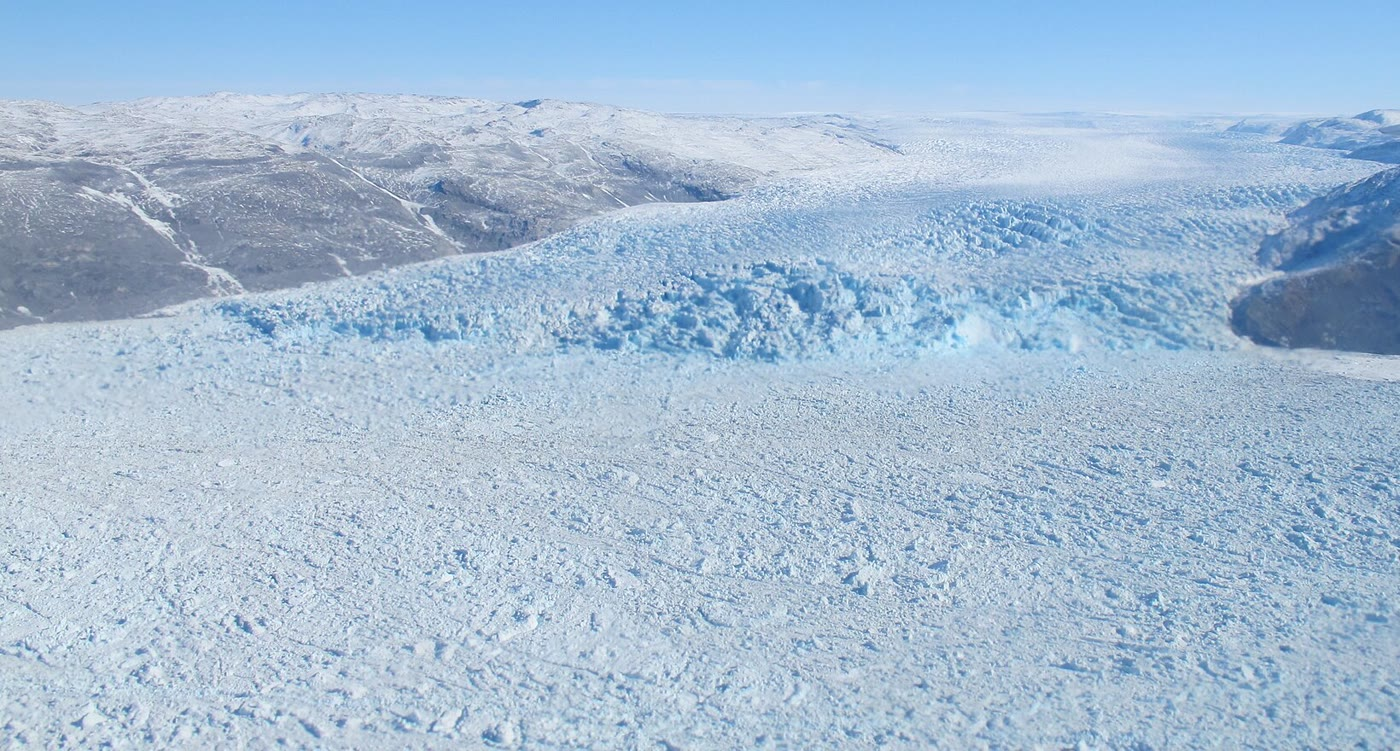
\includegraphics[width=0.82\linewidth]{images/book5/b3-greenland-outlet.jpg}

\par\smallskip{\small Un glacier émissaire de la calotte glaciaire du Groenland,
entre des montagnes, qui atteint la mer à son front de \omterm{def:b3:glaciology:grounding-line}{vêlage}, la paroi brisée
de glace bleue traversant le milieu de l'image~; le fjord au premier plan est
encombré de glace vêlée et de banquise. Photographié depuis un avion de
l'opération IceBridge de la NASA en avril 2014 (NASA / Jim Yungel, domaine
public).}\label{fig:b3:glaciology:outlet}
\end{omfigure}
% ledger: photo:b3-greenland-outlet

\begin{inthefield}[Un camp sur la glace]
\begin{minipage}[t]{0.55\linewidth}\vspace{0pt}
Sur une calotte glaciaire, les instruments des glaciologues se déplacent en
traîneau et logent sous des tentes. Pour mesurer la vitesse de la glace, ils
enfoncent un piquet dans la neige et y montent l'antenne d'un récepteur de
navigation par satellite. Les récepteurs utilisés en géodésie fixent une
position à quelques centimètres près, de sorte que des positions répétées sur
plusieurs semaines ou saisons donnent la vitesse et la direction de la glace, et que
la hauteur du piquet, mesurée à nouveau, donne l'amincissement ou l'épaississement de la glace sous lui.
\end{minipage}\hfill
\begin{minipage}[t]{0.42\linewidth}\vspace{0pt}
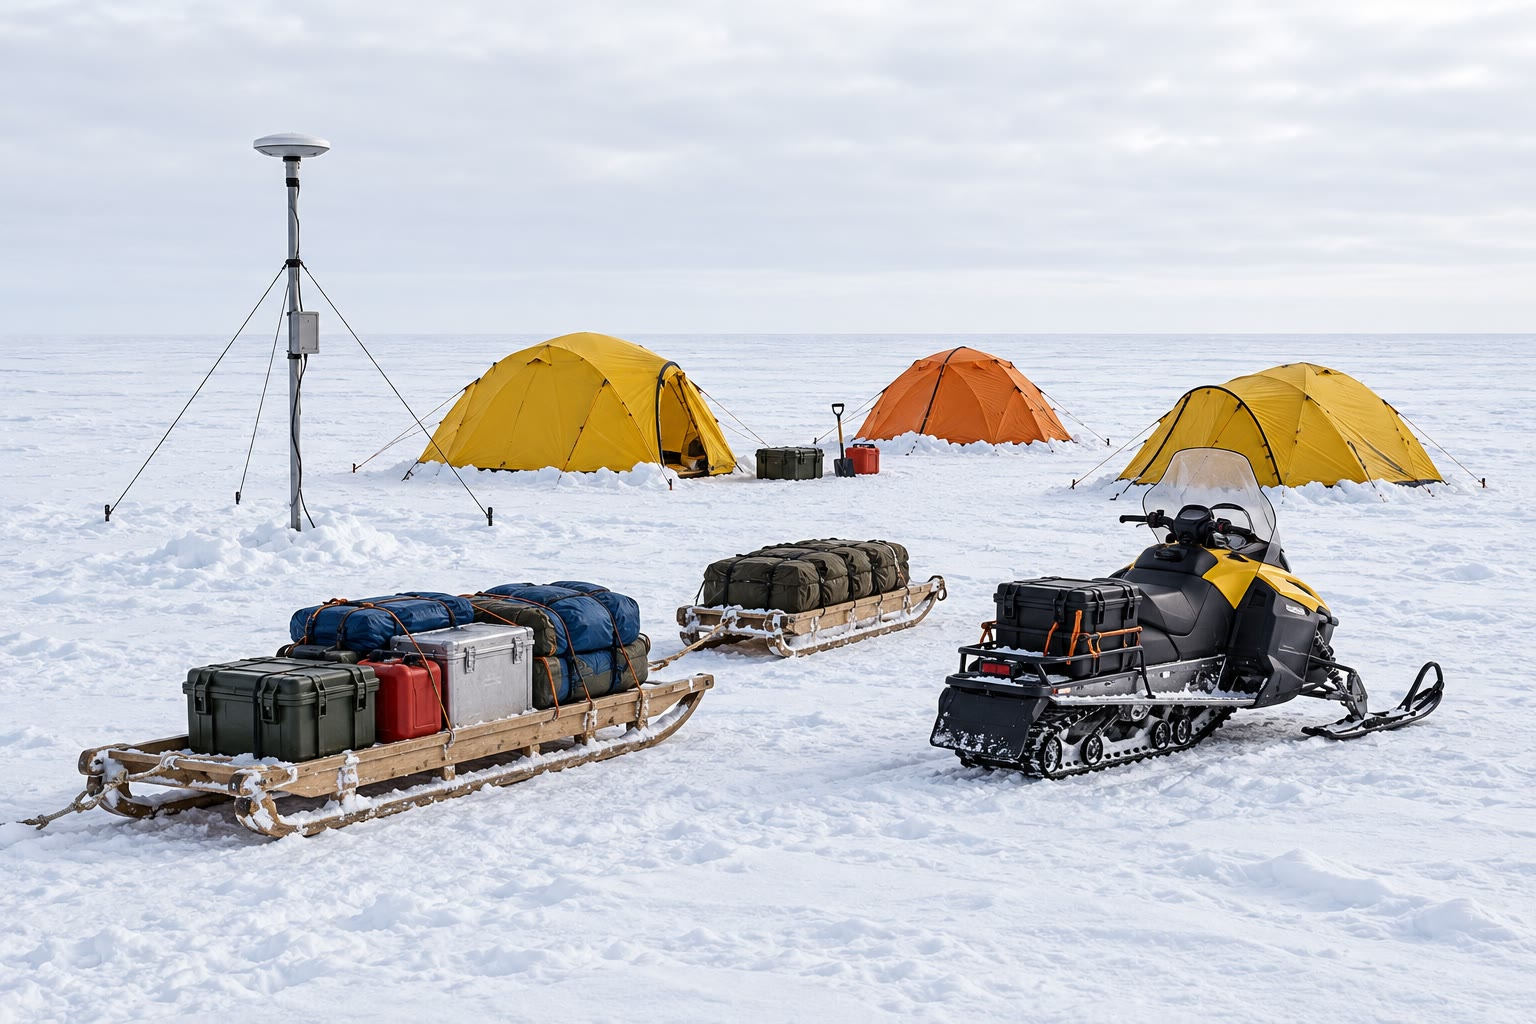
\includegraphics[width=\linewidth]{images/book5/ai/b3-glaciology-camp.jpg}

{\scriptsize Un camp de terrain sur une calotte glaciaire~: tentes, traîneaux et
motoneige, et antenne de navigation par satellite sur un mât maintenu par des
haubans (illustration générée par IA).}
\end{minipage}
\end{inthefield}
% ledger: gps:high-end

\section{Banquise et pergélisol}\label{sec:b3:glaciology:sea-ice}

La banquise se forme, croît et fond dans l'océan. En Arctique, elle atteint sa
plus grande étendue en mars et sa plus petite en septembre.
% ledger: nsidc:sea-ice-def

\begin{definition}[Étendue de la banquise]\label{def:b3:glaciology:sea-ice}
L'\emph{étendue de la banquise}\index{etendue@étendue de la banquise} est l'aire totale des
cellules d'une carte satellitaire où la banquise couvre plus de
\qty{15}{\percent} de la surface. Elle est supérieure à l'aire de la banquise,
qui ne compte que la glace elle-même.
\end{definition}
% ledger: nsidc:sea-ice-def

Depuis que les satellites la cartographient, à partir de 1979, l'étendue arctique
a diminué, en mars et bien davantage en septembre~: de \qty{0.74}{\mega km^2} par décennie en
septembre, soit environ \qty{12}{\percent} de la moyenne 1981--2010 par décennie, contre
\qty{0.38}{\mega km^2}, \qty{2.5}{\percent}, en mars. La plus petite étendue de
septembre observée jusqu'ici, \qty{3.57}{\mega km^2}, date de 2012. La banquise
arctique réfléchit \qtyrange{50}{70}{\percent} de la lumière solaire, l'océan
libre environ \qty{6}{\percent}~: la perte de glace assombrit la surface, c'est
la rétroaction glace--albédo du volume de deuxième année.
% ledger: data:b5-nsidc-extent, nsidc:sea-ice-reflect

La banquise croît à sa base, là où l'eau de mer gèle sur elle, et la chaleur latente
de cette congélation doit être conduite à travers la glace jusqu'à l'air froid.

\begin{theorem}[Loi de Stefan]\label{thm:b3:glaciology:stefan}
La banquise, de conductivité thermique $k_i$, de masse volumique $\rho_i$ et de chaleur
latente de fusion $L$, dont la surface est maintenue à une température $\Delta T$ sous le
point de congélation de l'eau sous-jacente, croît, si le flux de chaleur venant de l'océan
est négligeable, selon
\[
h(t)^2 - h(0)^2 = \frac{2k_i\,\Delta T}{\rho_iL}\,t .
\]
Sous une couche de neige d'épaisseur $h_s$ et de conductivité $k_s$, la vitesse de
croissance vaut $\mathrm dh/\mathrm dt = \Delta T/[\rho_iL(h/k_i + h_s/k_s)]$.
\end{theorem}

\begin{proof}
La température dans la glace mince est linéaire, depuis le point de congélation à la
base jusqu'à la température de surface au sommet, de sorte que le flux de chaleur qui la
traverse vaut $k_i\Delta T/h$, ou, à travers la glace et la neige en série, $\Delta T/(h/k_i +
h_s/k_s)$. La congélation d'une couche $\mathrm dh$ libère $\rho_iL\,\mathrm dh$ par
unité de surface, que ce flux doit évacuer~: $\rho_iL\,\mathrm dh/\mathrm dt
= k_i\Delta T/h$. Alors $\mathrm d(h^2)/\mathrm dt = 2k_i\Delta T/(\rho_iL)$.
\end{proof}

Avec $k_i = \qty{2.03}{W.m^{-1}.K^{-1}}$, $L = \qty{3.34e5}{J/kg}$ et
$\rho_i = \qty{917}{kg/m^3}$, une surface située \qty{20}{K} sous le point de congélation
forme \qty{1.5}{m} de glace en cent jours et \qty{2.1}{m} en deux cents jours.
La neige, de conductivité \qty{0.30}{W.m^{-1}.K^{-1}}, est un bon isolant~: \qty{20}{cm}
de neige réduisent plus que de moitié la croissance. La glace épaisse croît
lentement, la glace mince rapidement~: la loi tend à uniformiser l'épaisseur de la glace
après un été de fonte.
% ledger: cice:constants, iapws:ice-density

\begin{omfigure}
\begin{tikzpicture}
\begin{groupplot}[group style={group size=2 by 1, horizontal sep=1.5cm},
  width=0.48\linewidth, height=0.4\linewidth,
  tick label style={font=\scriptsize}, label style={font=\small}, title style={font=\small}]
\nextgroupplot[xlabel={année}, ylabel={étendue (\unit{\mega km^2})}, xmin=1977, xmax=2028,
  ymin=0, ymax=18, title={Étendue de la banquise arctique},
  xticklabel style={/pgf/number format/1000 sep={}},
  legend style={font=\scriptsize, at={(0.03,0.66)}, anchor=west}]
% computed in figdata/bachelor-3/sea_ice.py
\addplot[omDef, thick, mark=*, mark size=0.9pt] table[x=year, y=mar] {figdata/out/bachelor-3-sea_ice-extent.dat};
\addlegendentry{mars}
\addplot[omThm, thick, mark=*, mark size=0.9pt] table[x=year, y=sep] {figdata/out/bachelor-3-sea_ice-extent.dat};
\addlegendentry{septembre}
\addplot[black!60, densely dashed, forget plot] table[x=year, y=mar] {figdata/out/bachelor-3-sea_ice-trend.dat};
\addplot[black!60, densely dashed, forget plot] table[x=year, y=sep] {figdata/out/bachelor-3-sea_ice-trend.dat};
\nextgroupplot[xlabel={jours de gel}, ylabel={épaisseur de glace (\unit{m})}, xmin=0, xmax=200,
  ymin=0, ymax=2.4, title={Croissance, $\Delta T = \qty{20}{K}$},
  legend style={font=\scriptsize, at={(0.97,0.03)}, anchor=south east}]
\addplot[omMeth, thick] table[x=day, y=h0] {figdata/out/bachelor-3-sea_ice-stefan.dat};
\addlegendentry{glace nue}
\addplot[omDef, thick, densely dashed] table[x=day, y=hs] {figdata/out/bachelor-3-sea_ice-stefan.dat};
\addlegendentry{sous \qty{20}{cm} de neige}
\end{groupplot}
\end{tikzpicture}

\par\smallskip{\small À gauche, l'\omterm{def:b3:glaciology:sea-ice}{étendue de la banquise} arctique, en moyenne, en mars et en
septembre, de 1979 à 2026 (NSIDC Sea Ice Index, version~4), avec les tendances par
moindres carrés (pointillés)~: \qty{-0.38}{\mega km^2} et \qty{-0.74}{\mega km^2} par
décennie. À droite, la croissance de la banquise par conduction sous une surface située
\qty{20}{K} sous le point de congélation, sans chaleur océanique~: la glace nue selon la
loi de Stefan, et la même glace sous \qty{20}{cm} de neige.}\label{fig:b3:glaciology:sea-ice}
\end{omfigure}
% ledger: data:b5-nsidc-extent, cice:constants

Le pergélisol est le sol qui reste à \qty{0}{\celsius} ou en dessous pendant deux
ans ou plus. Il sous-tend environ un quart des terres émergées de l'hémisphère Nord.
l'hémisphère Nord.
% ledger: nsidc:permafrost

\begin{definition}[Couche active]\label{def:b3:glaciology:permafrost}
La \emph{couche active}\index{couche active} est la couche de sol située au-dessus du
pergélisol, qui dégèle chaque été et regèle chaque hiver.
\end{definition}

Son épaisseur est déterminée, comme la croissance de la banquise, par la conduction de
la chaleur dans le sol pendant la saison de dégel, contre la chaleur latente de la glace
du sol. Les températures du pergélisol ont augmenté au cours des trois à quatre dernières
décennies dans l'ensemble des régions de pergélisol (confiance élevée)~;
le pergélisol s'est réchauffé à l'échelle mondiale de \qty{0.29}{\celsius} [\numrange{0.17}{0.41}]
entre 2007 et 2016 (confiance moyenne), et l'augmentation de l'épaisseur de la \omterm{def:b3:glaciology:permafrost}{couche active}
est un phénomène panarctique (confiance moyenne). Là où sa glace fond, le sol peut
s'effondrer.
% ledger: ar6ch9:permafrost, nsidc:permafrost-thaw

\section{La cryosphère et le niveau de la mer}\label{sec:b3:glaciology:sea-level}

Le bilan du niveau marin du volume de deuxième année ajoute l'expansion de l'océan qui se
réchauffe à l'eau apportée par la glace et par les terres. Sur les
\qty{3.69}{mm/an} d'élévation du niveau de la mer observés entre 2006 et 2018, les glaciers
ont contribué pour \qty{0.62}{mm/an}, le Groenland pour \qty{0.63}{mm/an} et l'Antarctique
pour \qty{0.37}{mm/an}~: la glace, prise ensemble, dépasse l'expansion de l'océan,
\qty{1.39}{mm/an}.
% ledger: ar6ch9:table95

\begin{dated}{2021}
Le Groenland a perdu \qty{4890}{Gt} de glace entre 1992 et 2020 [4140 à 5640],
soit \qty{13.5}{mm} de niveau marin, à des rythmes passés de \qty{39}{Gt/an} dans les
années 1990 à \qty{243}{Gt/an} entre 2010 et 2019, par débit et, de plus en plus,
par fonte de surface (confiance élevée). L'Antarctique a perdu \qty{2670}{Gt}
[1800 à 3540], soit \qty{7.4}{mm}, son rythme passant de \qty{49}{Gt/an} dans les années
1990 à \qty{148}{Gt/an} entre 2010 et 2019~; les pertes proviennent des glaciers émissaires de
l'Antarctique occidental, principalement par la fonte des plates-formes de glace par-dessous (confiance
élevée). Les glaciers hors des calottes glaciaires ont perdu \qty{6200}{Gt} entre
1993 et 2019, soit \qty{17.1}{mm}, davantage entre 2010 et 2019 que dans toute autre décennie
de la série (confiance très élevée). Le Groenland continuera de perdre de la masse
tout au long de ce siècle selon tous les scénarios considérés (quasi
certain), et l'Antarctique aussi (probable)~: d'ici 2100, le Groenland ajoutera
probablement \qtyrange{0.01}{0.10}{m} au niveau de la mer dans un scénario de faibles
émissions et \qtyrange{0.09}{0.18}{m} dans un scénario de très fortes émissions,
l'Antarctique \qtyrange{0.03}{0.27}{m} et \qtyrange{0.03}{0.34}{m}. L'océan Arctique
deviendra probablement pratiquement libre de banquise, avec moins de
\qty{1}{\mega km^2} à son minimum de septembre, pour la première fois avant 2050 selon
tous les scénarios considérés.
\end{dated}
% ledger: ar6ch9:greenland, ar6ch9:antarctica, ar6ch9:glaciers, ar6ch9:ice-sheet-proj, ar6ch9:sea-ice

Les pertes des calottes glaciaires sont celles du chapitre~\ref{ch:b3:gravity-geodesy},
mesurées par altimétrie, par gravimétrie et par la différence entre la neige
qui tombe et la glace qui s'écoule~: trois méthodes indépendantes
réunies en une seule estimation.
% ledger: data:b5-imbie

\section{Exercices}

\begin{exercise}[$\star$]\label{exo:b3:glaciology:1}
Une vallée glaciaire épaisse de \qty{250}{m} s'écoule sur une pente de \ang{3}. Calculer
la contrainte de cisaillement basale, et la comparer aux contraintes basales de
glaciers réels, de l'ordre du bar.
\end{exercise}

\begin{exercise}[$\star$]\label{exo:b3:glaciology:2}
(a)~La calotte glaciaire du Groenland contient environ \qty{2.9}{\mega km^3} de glace de
masse volumique \qty{917}{kg/m^3}. Calculer sa masse et son \omterm{def:b3:glaciology:sle}{équivalent en niveau marin} à
\qty{360}{Gt/mm}, et comparer avec les \qty{7.4}{m} généralement cités.
(b)~Faire de même pour les \qty{30}{\mega km^3} de l'Antarctique, cités comme environ
\qty{58}{m}. Pourquoi les deux se comparent-elles si différemment~?
\end{exercise}
% ledger: nsidc:ice-sheets

\begin{exercise}[$\star$]\label{exo:b3:glaciology:3}
Un glacier possède une \omterm{def:b3:glaciology:mass-balance}{zone d'accumulation} de \qty{6}{km^2} avec un bilan moyen de
\qty{+1.2}{m} d'équivalent en eau, et une \omterm{def:b3:glaciology:mass-balance}{zone d'ablation} de \qty{4}{km^2} avec
\qty{-2.1}{m}. Calculer son bilan net en mètres cubes d'eau, son bilan
spécifique moyen, et son rapport de surface d'accumulation. Grandit-il ou
diminue-t-il~?
\end{exercise}

\begin{exercise}[$\star$]\label{exo:b3:glaciology:4}
À la \omterm{def:b3:glaciology:firn}{fermeture des pores}, le \omterm{def:b3:glaciology:firn}{névé} a une masse volumique de \qtyrange{820}{830}{kg/m^3}.
Quelle fraction de son volume reste occupée par les pores (glace~:
\qty{917}{kg/m^3})~?
\end{exercise}
% ledger: firn:close-off

\begin{exercise}[$\star\star$]\label{exo:b3:glaciology:5}
Un glacier tempéré (glace à \qty{0}{\celsius}, $A =
\qty{1.4e-16}{Pa^{-3}.an^{-1}}$) a une épaisseur de \qty{300}{m} sur une pente de
\ang{3}. Calculer sa vitesse de surface due à la seule déformation interne. De quel
facteur la vitesse changerait-elle s'il était deux fois plus épais~? Et si la pente
était divisée par deux~?
\end{exercise}

\begin{exercise}[$\star\star$]\label{exo:b3:glaciology:6}
À partir des constantes de Paterson--Budd, calculer le \omterm{def:b3:glaciology:glen}{coefficient de fluage} à
\qty{-25}{\celsius} et à \qty{-10}{\celsius}, ainsi que le rapport des vitesses de
deux masses de glace identiques à \qty{0}{\celsius} et à \qty{-25}{\celsius}.
\end{exercise}
% ledger: pism:rheology, codata:R

\begin{exercise}[$\star\star$]\label{exo:b3:glaciology:7}
Calculer l'épaisseur maximale d'une calotte de glace plastique de \qty{1000}{km} du
centre à la marge, avec $\tau_0 = \qty{100}{kPa}$, et comparer avec l'épaisseur
maximale de la glace antarctique, voisine de \qty{4.9}{km}.
\end{exercise}
% ledger: nsidc:ice-sheets

\begin{exercise}[$\star\star$]\label{exo:b3:glaciology:8}
Un glacier épais de \qty{200}{m} perd \qty{5}{m} de glace par an à son front.
Estimer son temps de réponse. Si le climat se réchauffe brusquement puis reste
stable, pendant combien de temps sa longueur continuerait-elle à changer~?
\end{exercise}

\begin{exercise}[$\star\star$]\label{exo:b3:glaciology:9}
(a)~En utilisant la loi de Stefan avec $\Delta T = \qty{20}{K}$, calculer l'épaisseur
de la banquise nue après \num{100}~jours, et le temps nécessaire pour atteindre \qty{3}{m}.
(b)~Que suggère ce résultat pour la glace plus épaisse que \qty{3}{m}~?
\end{exercise}
% ledger: cice:constants

\begin{exercise}[$\star\star\star$]\label{exo:b3:glaciology:10}
(a)~Là où le lit se trouve à \qty{800}{m} sous le niveau de la mer, quelle est
l'épaisseur de la glace à la \omterm{def:b3:glaciology:grounding-line}{ligne d'échouage}~? (b)~En utilisant le flux de panneau
$q \propto H^{n+2}$ pour une pente de surface donnée, de quel facteur le flux de la
glace posée augmente-t-il si la \omterm{def:b3:glaciology:grounding-line}{ligne d'échouage} recule jusqu'à un lit à \qty{900}{m} de profondeur~? (c)~Expliquer
pourquoi un lit qui s'approfondit vers l'intérieur rend le recul auto-renforçant, et ce que
change une plate-forme de glace.
\end{exercise}
% ledger: iapws:ice-density, noaa:seawater-1025

\begin{exercise}[$\star\star\star$]\label{exo:b3:glaciology:11}
Montrer que le volume d'une calotte plastique circulaire de rayon $R$ vaut $V =
\frac{8\pi}{15}\sqrt{2\tau_0/(\rho g)}\,R^{5/2}$. De quel facteur son \omterm{def:b3:glaciology:sle}{équivalent en
niveau marin} augmente-t-il si son rayon double~?
\end{exercise}

\begin{exercise}[$\star\star\star$]\label{exo:b3:glaciology:12}
L'étendue moyenne de l'Arctique était de \qty{16.34}{\mega km^2} en mars 1979 et
de \qty{14.13}{\mega km^2} en mars 2026~; en septembre, \num{7.05} et
\qty{4.81}{\mega km^2}. (a)~Calculer la variation relative pour chaque mois.
(b)~Donner deux raisons physiques pour lesquelles l'étendue de septembre a autant
diminué plus vite que celle de mars.
\end{exercise}
% ledger: data:b5-nsidc-extent

\section{Problème~: la calotte d'Arkel}

\begin{problem}[{Problème du week-end --- la forme, l'écoulement, le bilan et
l'équivalent en niveau marin d'une calotte inventée}]
\label{pb:b3:glaciology:1}
La calotte inventée d'Arkel repose sur un plateau plat. Elle est presque circulaire,
de \qty{20}{km} de rayon, et sa glace est à environ \qty{-10}{\celsius}. Prendre
$\rho = \qty{917}{kg/m^3}$ et $g = \qty{9.81}{m/s^2}$.

\medskip\noindent\textbf{Partie I --- La calotte est-elle plastique~?}
\begin{enumerate}
\item Montrer que, sous une glace d'épaisseur $H$ avec une faible pente de surface
  $\alpha$, la contrainte de cisaillement basale vaut environ $\rho gH\alpha$.
\item Les sondages radar et les relevés à 5, 10 et \qty{15}{km} du centre donnent
  des épaisseurs de 580, 470 et \qty{335}{m} et des pentes de surface de
  \num{0.0190}, \num{0.0240} et \num{0.0330}. Calculer la contrainte de cisaillement
  basale aux trois points.
\item La calotte est-elle proche d'un comportement plastique~? Quelle limite d'écoulement retenir~?
\item Avec $\tau_0 = \qty{100}{kPa}$, calculer $2\tau_0/(\rho g)$.
\item Prédire l'épaisseur aux trois points à partir du profil plastique
  et comparer avec les sondages.
\end{enumerate}

\medskip\noindent\textbf{Partie II --- Forme et volume.}
\begin{enumerate}[resume]
\item Calculer l'épaisseur au centre.
\item Montrer que le volume vaut $V = \frac{8\pi}{15}\sqrt{2\tau_0/(\rho
  g)}\,R^{5/2}$.
\item Calculer le volume en kilomètres cubes.
\item Calculer la surface et l'épaisseur moyenne.
\item Une calotte deux fois plus large sur le même plateau~: de quel facteur son
  volume est-il plus grand~?
\end{enumerate}

\medskip\noindent\textbf{Partie III --- Écoulement et bilan.}
\begin{enumerate}[resume]
\item Calculer le \omterm{def:b3:glaciology:glen}{coefficient de fluage} à \qty{-10}{\celsius} en
  \unit{Pa^{-3}.an^{-1}}.
\item À \qty{10}{km} du centre, en assimilant la glace à une dalle, calculer la
  vitesse de surface due à la déformation interne.
\item Calculer le flux de glace par unité de largeur en ce point, ainsi que la
  vitesse moyenne de la colonne.
\item En régime stationnaire, le flux qui sort du cercle de rayon
  \qty{10}{km} est égal au bilan gagné à l'intérieur de celui-ci. Quel bilan
  moyen, en mètres de glace par an, cela impose-t-il~?
\item La ligne d'équilibre se situe \qty{450}{m} au-dessus du plateau. Où se
  trouve-t-elle sur la calotte, et quel est le rapport de la \omterm{def:b3:glaciology:mass-balance}{zone d'accumulation}~?
\item Si la glace se réchauffait jusqu'à \qty{0}{\celsius}, de quel facteur les
  vitesses augmenteraient-elles~? Que deviendrait la forme de la calotte~?
\end{enumerate}

\medskip\noindent\textbf{Partie IV --- Niveau de la mer.}
\begin{enumerate}[resume]
\item Calculer la masse de la calotte en gigatonnes.
\item Calculer son \omterm{def:b3:glaciology:sle}{équivalent en niveau marin} en millimètres.
\item Si la calotte entière s'amincissait de \qty{0.5}{m} de glace par an, sans
  s'écouler, combien de temps durerait-elle~?
\item Pourquoi la calotte réelle disparaîtrait-elle plus vite que cela, une fois
  qu'elle commencerait à s'amincir~?
\item Au rythme auquel le Groenland a perdu de la glace entre 2010 et 2019, combien
  de temps faudrait-il pour perdre une masse égale à celle de la calotte d'Arkel~?
\item Donner l'\omterm{def:b3:glaciology:sle}{équivalent en niveau marin} de la calotte glaciaire d'Arkel, en
  millimètres, à un chiffre après la virgule.
\end{enumerate}
\end{problem}
% ledger: pism:rheology, data:b5-imbie, ar6ch9:greenland, ar6ch9:faq91
